\documentclass[12pt]{article}
\usepackage{graphicx}

\begin{document}

\huge Use Case Details

\begin{itemize}

\item \large Create Employee\\
Figure 1 depicts how an applicant applies to be a broker, and how the Manager is involved in the process.

\begin{figure}[h]
\centering
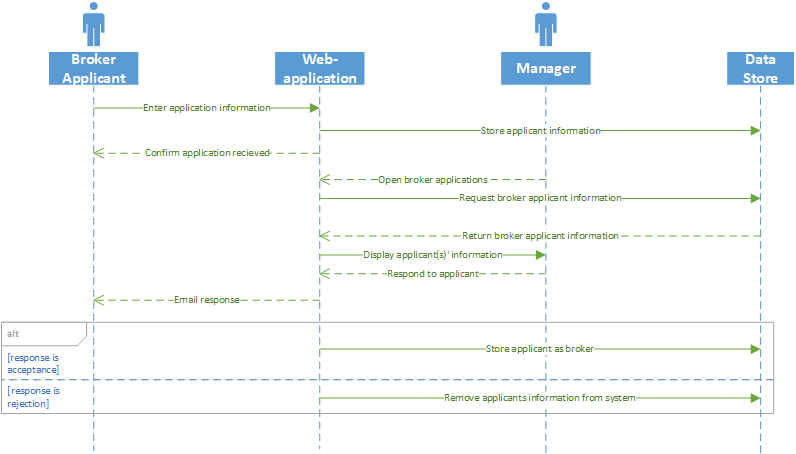
\includegraphics[scale=0.8]{SSDCreateEmployeeV1}
\caption{System Sequence Diagram (SSD) for the 'Create Employee' use case}
\end{figure}


\item \large Create Home Application\\
Figure 2 depicts the steps taken by customer to create a new home application.

\begin{figure}[h]
\centering
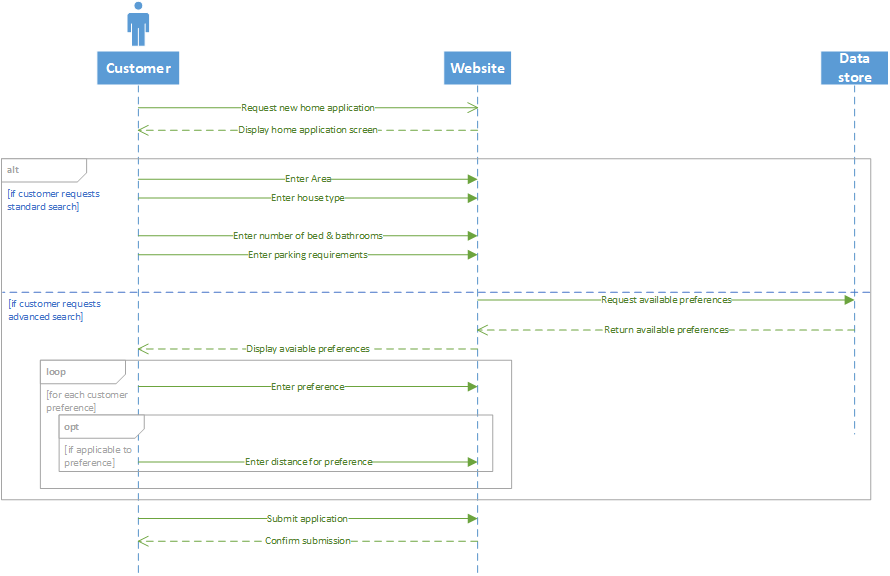
\includegraphics[scale=0.7]{SSDCreateHomeApplication}
\caption{System Sequence Diagram for the 'Create Home Application' use case}
\end{figure}

\item Create Home Suggestion\\
The above use case involves the 3 main parts: the system, the application (includes the customer preferences) and the Google Maps API (GMAPI).\\
After the customer has made an application for a smart home selection, the system will request the location of all the customers preferences in the vicinity of the customers preferred area from the GMAPI (for example, if the customer wanted a nearby hospital and to live in Sandton, all the hospitals near Sandton would be retrieved).\\
From there, the System will retrieve all the available homes in the relevant area and will cross reference them with the applications preferences.

\item Home Management\\

\item Transaction Management

\end{itemize}
\end{document}